\documentclass{report}

\usepackage{graphicx} % Add pictures to your document
\usepackage{float}

\begin{document}

\title{\huge{\textbf{iPantry}} \\ Grupo 403 \\ BDAD 2019/2020 \\ MIEIC FEUP}
\author{João de Jesus Costa \\ \texttt{up201806560} \and
	João Lucas Silva Martins \\ \texttt{up201806436} \and
	Tiago Duarte da Silva \\ \texttt{up201806516}}
\date{\today{}}

\begin{figure}[b]
	\centering
	
\includegraphics[width=0.6\textwidth]{feup_logo.png}
\end{figure}
\maketitle{}

\tableofcontents{}
\newpage

\newcommand{\foreign}[2] {$\hbox{#1} \rightarrow \hbox{#2}$}

\newcommand{\foreignkey}[2] {$\hbox{\underline{#1}} \rightarrow \hbox{#2}$}

\chapter{Objetivo}
Precedemos simular um sistema centralizado que permita vários utilizadores manter
um inventário atualizado de todos os produtos que têm nas suas despensas.
\newline
O utilizador pode listar o conteúdo da sua despensa, filtrar/procurar produtos por
(sub-)categoria e/ou nome e realizar encomendas em lojas que o permitam. Estas
encomendas podem ser automáticas, no caso de produtos considerados `vitais', ou
espontâneas (a pedido do utilizador). Para realizar uma encomenda o utilizador
apenas necessita de criar uma lista de produtos que pretende comprar, sendo que
a aplicação irá comprá-los nos locais `mais em conta'.
\newline
Produtos `vitais' são produtos que irão gerar notificações quando a sua quantidade
em inventário chega ao nível mínimo predefinido pelo utilizador. Também é possível
marcar um produto `vital' para renovação automática, ou seja, sempre que o inventário
deste for baixo (tendo em conta as preferências do utilizador), este será
encomendado/comprado automaticamente.
\newline
O histórico de encomendas/compras de cada utilizador permite a sugestão de produtos
por parte da aplicação.

\chapter{Especificação}
\section{Despensa}
Cada despensa (uma despensa representa um cliente) tem nome, morada,
código postal, os produtos do utilizador em inventário e o seu histórico
de encomendas/compras. Para cada um destes produtos é registada a quantidade
atualmente disponível, se este é considerado um produto `vital' e, nesse caso,
a quantidade mínima a manter em inventário e se este deve ser
comprado/encomendado de forma automática.

\section{Produtos}
Sobre cada produto é guardado o nome, o código de barras (caso exista), as suas
categorias e subcategorias, as lojas onde pode ser comprado e o respetivo preço
em cada uma dessas.
\subsection{Categorias de Produtos}
Cada produto tem que pertencer a pelo menos uma categoria (principal) e pode
pertencer a diversas subcategorias. As categorias e subcategorias são
hierarquizadas, por exemplo: \foreign{Bebida}{Refrigerante, Sumo, Bebidas Alcoólicas};
\foreign{Bebidas Alcoólicas}{Vinho, Cerveja, Bebidas Espirituosas}.

\section{Encomendas}
Cada encomenda possui um identificador único, uma data de emissão, um montante,
uma loja em que foi feita a encomenda, e uma lista dos produtos comprados e em
que quantidades.

\section{Lojas}
Cada loja tem nome, morada, código postal, e uma lista de produtos que vende
com os seus respetivos preços sem descontos associados.
\newline
Uma loja pode (no máximo) fazer parte de uma cadeia de lojas.
\subsection{Cadeia de lojas}
Uma cadeia de lojas é uma composição de diversas lojas. Estas têm um nome
e uma lista de descontos associada a um ou mais produtos. Todas as lojas
associadas a uma cadeia de lojas têm de aplicar a lista de descontos da sua
cadeia aos seus produtos.
\newline
No caso de não pertencer a nenhuma cadeia de lojas, uma loja pode ter a sua
própria lista de descontos a aplicar aos seus produtos.
\subsection{Descontos}
Um desconto tem uma percentagem (quantidade de desconto), uma data de ínicio
da promoção, uma data de fim da promoção e uma lista de produtos em que é
aplicável.

\chapter{Modelo conceptual}
\begin{figure}[H]
	\centering
	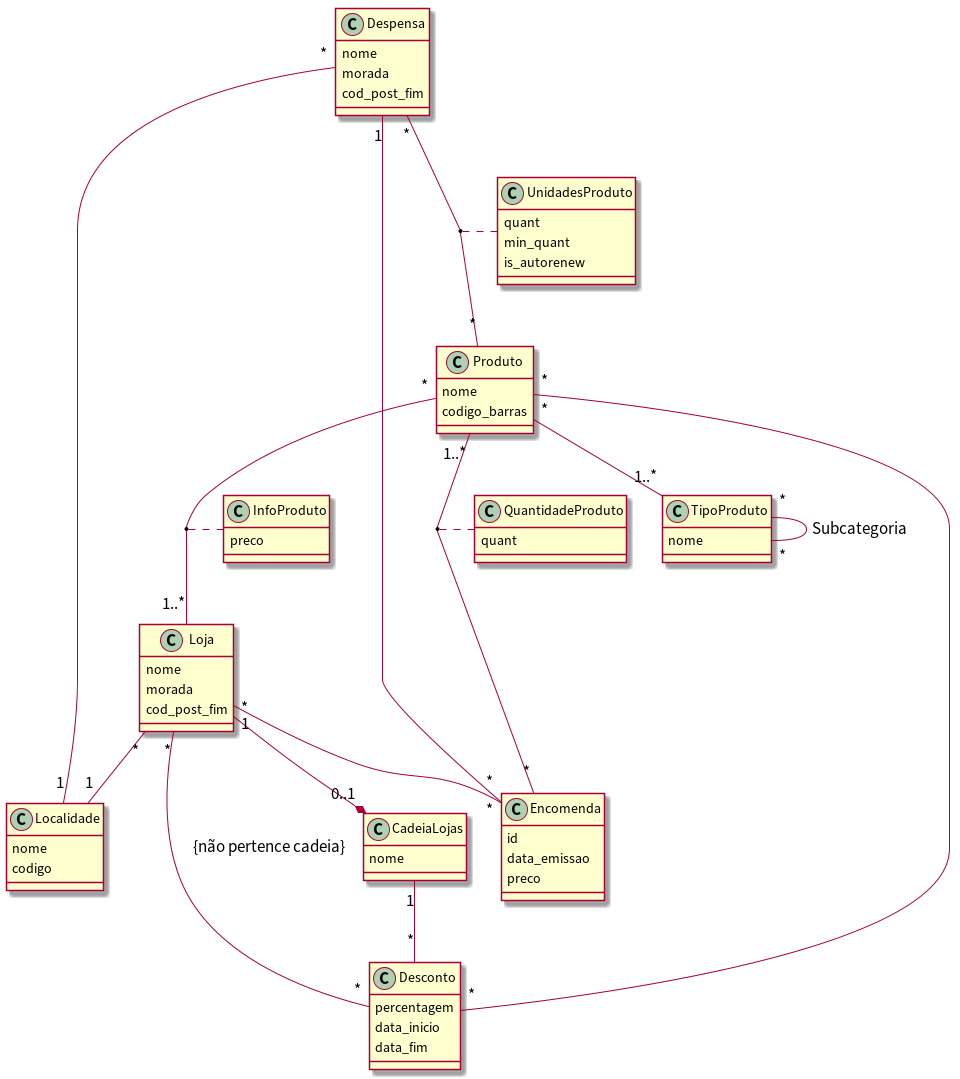
\includegraphics[width=0.9\textwidth]{../uml_model/modelo_concpt.png}
\end{figure}

\chapter{Modelo conceptual (Revisto)}
\begin{figure}[H]
	\centering
	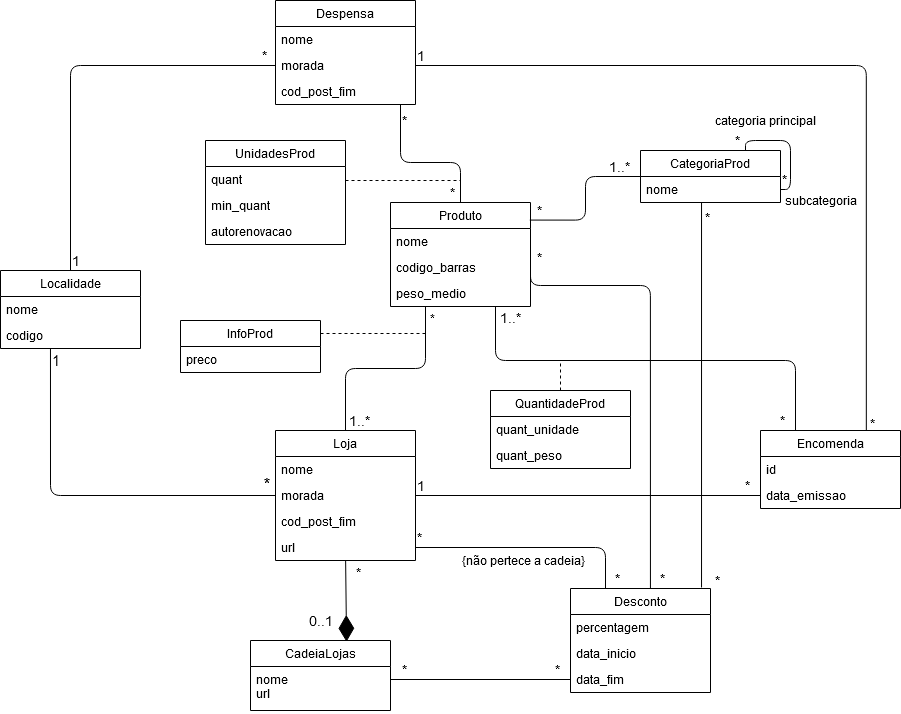
\includegraphics[width=0.9\textwidth]{../uml_model/modelo_concpt_revised.png}
\end{figure}

\chapter{Modelo relacional e dependências funcionais}
\section{Modelo relacional}
\textbf{Despensa} (\underline{id}, nome, morada, cod\_post\_fim,
\foreign{id\_localidade}{Localidade})\\\\

\textbf{Produto} (\underline{id}, codigo\_barras, nome, peso\_medio)\\\\

\textbf{CategoriaProd} (\underline{id}, nome)\\\\

\textbf{Loja} (\underline{id}, nome, morada, cod\_post\_fim, url,
\foreign{id\_localidade}{Localidade}, \foreign{id\_cadeia}{CadeiaLojas})\\\\

\textbf{CadeiaLojas} (\underline{id}, nome, url)\\\\

\textbf{Encomenda} (\underline{id}, data\_emissao, \foreign{id\_despensa}{Despensa},
\foreign{id\_loja}{Loja})\\\\

\textbf{Desconto} (\underline{id}, percentagem, data\_inicio, data\_fim)\\\\

\textbf{Localidade} (\underline{id}, codigo, nome)\\\\

\textbf{UnidadesProduto} (\foreignkey{id\_despensa}{Despensa},
\foreignkey{id\_produto}{Produto}, quant, min\_quant, autorenovacao)\\\\

\textbf{InfoProduto} (\foreignkey{id\_produto}{Produto},
\foreignkey{id\_loja}{Loja}, preco)\\\\

\textbf{QuantidadeProd} (\foreignkey{id\_produto}{Produto},
\foreignkey{id\_encomenda}{Encomenda}, quant\_unidade, quant\_peso)\\\\

\textbf{Categoria} (\foreignkey{id\_produto}{Produto},
\foreignkey{id\_categoria}{CategoriaProd})\\\\

\textbf{SubCategoria} (\foreignkey{id\_categoria\_mae}{CategoriaProd},
\foreignkey{id\_subcategoria}{CategoriaProd})\\\\

\textbf{CategoriaDesconto} (\foreignkey{id\_categoria}{CategoriaProd},
\foreignkey{id\_desconto}{Desconto})\\\\

\textbf{ProdutoDesconto} (\foreignkey{id\_produto}{Produto},
\foreignkey{id\_desconto}{Desconto})\\\\

\textbf{LojaDesconto} (\foreignkey{id\_loja}{Loja},
\foreignkey{id\_desconto}{Desconto})\\\\

\textbf{CadeiaDesconto} (\foreignkey{id\_cadeia}{CadeiaLojas},
\foreignkey{id\_desconto}{Desconto})\\\\

\section{Dependências funcionais}

\subsection{Despensa}
\foreign{id}{nome, morada, cod\_post\_fim, id\_localidade}\\
\foreign{nome}{id, morada, cod\_post\_fim, id\_localidade}\\
\newline
Chaves da relação: \{id\} e \{nome\}\\
Está na BCNF pois tanto \{id\} como \{nome\} são chaves candidatas. Por
consequência, está na 3NF, pois está na BCNF.

\subsection{Produto}
\foreign{id}{codigo\_barras, nome, peso\_medio}\\
\newline
Chaves da relação: \{id\}\\
Está na BCNF pois \{id\} é a chave mínima. Está na forma 3NF, dado que está
na BCNF.\\
É de notar que apesar do \textbf{código\_barras} ser único, não é chave
da relação, pois nem todos os produtos têm um código de barras (e.g.:
produtos internos de uma loja).

\subsection{CategoriaProd}
\foreign{id}{nome}\\
\foreign{nome}{id}\\
\newline
Chaves da relação: \{id\} e \{nome\}\\
Está na BCNF pois \{id\} e \{nome\} são chaves da relação. Está na 3NF,
dado que está na BCNF.

\subsection{Loja}
\foreign{id}{nome, morada, cod\_post\_fim, url, id\_localidade, id\_cadeia}\\
\foreign{nome, morada, cod\_post\_fim, url, id\_localidade, id\_cadeia}{id}\\
\newline
Chaves da relação: \{id\} e \{nome, morada, cod\_post\_fim, url,
id\_localidade, id\_cadeia\}\\
Está na BCNF, pois \{id\} e \{nome, morada, cod\_post\_fim, url,
id\_localidade, id\_cadeia\} são chaves da relação. Está na 3NF,
dado que está na BCNF.

\subsection{CadeiaLojas}
\foreign{id}{nome, url}\\
\foreign{nome}{id, url}\\
\foreign{url}{id, nome}\\
\newline
Chaves da relação: \{id\}, \{nome\} e \{url\}\\
Está na BCNF, pois todos os atributos da relação dependem funcionalmente
de uma chave. Por consequência, também está na 3NF.

\subsection{Encomenda}
\foreign{id}{data\_emissao, id\_despensa, id\_loja}\\
\foreign{data\_emissao, id\_despensa, id\_loja}{id}\\
\newline
Chaves da relação: \{id\} e \{data\_emissao, id\_despensa, id\_loja\}\\
Está na BCNF, pois \{id\} e \{data\_emissao, id\_despensa, id\_loja\} são
chaves da relação. Está na 3NF pois está na BCNF.\\
É de notar que a seguinte dependência funcional não existe nesta relação
pois podem haver duas encomendas diferentes no mesmo dia, feita pela mesma
despensa na mesma loja:\\
\foreign{data\_emissao, id\_despensa, id\_loja}{id}

\subsection{Desconto}
\foreign{id}{percentagem, data\_inicio, data\_fim}\\
\foreign{percentagem, data\_inicio, data\_fim}{id}\\
\newline
Chaves da relação: \{id\} e \{percentagem, data\_inicio, data\_fim\}\\
Esta relação está na BCNF, porque todos os seus atributos dependem funcionalmente
de uma (super-)chave da relação. Por consequência, esta relação também
está na 3NF.

\subsection{Localidade}
\foreign{id}{codigo, nome}\\
\foreign{nome}{codigo, id}
\newline
Chaves da relação: \{id\} e \{nome\}\\
Está na BCNF, pois \{id\} e \{nome\} são chaves candidatas da relação. Está
na 3NF pois está na BCNF.

\subsection{UnidadesProduto}
\foreign{id\_despensa, id\_produto}{quant, min\_quant, autorenovacao}\\
\newline
Chaves da relação: \{id\_despensa, id\_produto\}\\
Está na BCNF, pois \{id\_despensa, id\_produto\} é a chave mínima da relação.
Está na 3NF, pois também está na BCNF.

\subsection{InfoProduto}
\foreign{id\_produto, id\_loja}{preco}\\
\newline
Chaves da relação: \{id\_produto, id\_loja\}\\
Está na BCNF pois \{id\_produto, id\_loja\} é a chave mínima da relação. Está
na 3NF, pois também está na BCNF.\\

\subsection{QuantidadeProduto}
\foreign{id\_produto, id\_encomenda}{quant\_unidade, quant\_peso}\\
\newline
Chaves da relação: \{id\_produto, id\_encomenda\}\\
Está na BCNF pois \{id\_produto, id\_encomenda\} é a chave mínima da relação. Está
na 3NF, pois também está na BCNF.\\

\subsection{Categoria}
Não existem dependências funcionais nesta relação.

\subsection{SubCategoria}
Não existem dependências funcionais nesta relação.

\subsection{CategoriaDesconto}
Não existem dependências funcionais nesta relação.

\subsection{ProdutoDesconto}
Não existem dependências funcionais nesta relação.

\subsection{LojaDesconto}
Não existem dependências funcionais nesta relação.

\subsection{CadeiaDesconto}
Não existem dependências funcionais nesta relação.

\chapter{Restrições}
\section{Despensa}
Todas as despensas têm um id único, não nulo -- `PRIMARY KEY'.\\
Todas as despensas têm de ter um nome único, não nulo (`username`).\\
Os códigos postais são números positivos.\\
Uma despensa pode não ter uma morada. Nesse caso, os 3 campos referentes à morada
(morada, cod\_post\_fim e id\_localidade) devem ser nulos.
\section{Produto}
Todos os produtos têm um id único, não nulo -- `PRIMARY KEY'.\\
Todos os produtos têm de ter um nome (não nulo).\\
O código de barras de um produto, caso exista, tem de ser único.
\section{CategoriaProd}
Todas as categorias de produtos têm um id único, não nulo -- `PRIMARY KEY'.\\
Todas as categorias de produtos têm de ter um nome único, não nulo.
\section{Loja}
Todas as lojas têm um id único, não nulo -- `PRIMARY KEY'.\\
Todas as lojas têm de ter um nome (não nulo).\\
Uma loja só tem uma URL quando não faz parte de uma cadeia de lojas. Caso não
faça parte de uma cadeia de lojas, uma loja deverá ter uma URL única.\\
Os 'URL` são únicos.\\
Os códigos postais, caso exitam, são números positivos.\\
Uma loja pode não ter uma localização física. Nesse caso, os 3 campos referentes
à morada (morada, cod\_post\_fim e id\_localidade) devem ser nulos.\\
\section{CadeiaLojas}
Todas as cadeias de lojas têm um id único, não nulo -- `PRIMARY KEY'.\\
Todas as cadeias de lojas têm de ter um nome único, não nulo.\\
Todas as cadeias de lojas têm de ter uma `URL' única, não nula.
\section{Encomenda}
Todas as encomendas têm um id único, não nulo -- `PRIMARY KEY'.\\
Todas as encomendas têm uma data de emissão (não nula).\\
Todas as encomendas têm de pertencer a uma despensa e ter sido feitas numa
loja (chave estrangeira não nula).
\section{Desconto}
Todos os descontos têm um id único, não nulo -- `PRIMARY KEY'.\\
Todos os descontos têm de ter uma percentagem (não nula). Esta percentagem
tem de ser menor ou igual a 100 (\%).\\
Todos os descontos tem uma data de inicio da promoção (não nula). No entanto,
descontos podem não ter uma data de fim.\\
A data de fim de uma promoção (caso exista) tem de ser referente a um momento
posterior à data de inicio.
\section{Localidade}
Todas as localidades têm um código positivo, não necessariamente único (i.e.:
primeiros quatro dígitos do código postal).\\
Todas as localidades têm um nome único.\\
Tanto o código como o nome não podem ser nulos, e o seu identificar deverá
ser único e não nulo -- PRIMARY KEY.
\section{UnidadesProduto}
Os produtos existem em quantidades maiores ou iguais a 0. O mesmo se aplica à
quantidade mínima a manter em `stock`. Um produto tem que ter valor de
autorenovacao (não nulo).\\
A informação relativa à renovação automática de um produto não pode ser nula.\\
O par de identificadores da despensa e do produto são únicos e não nulos -- PRIMARY KEY.
\section{InfoProduto}
Os produtos têm preços maiores ou iguais a 0.
O par de identificadores do produto e da loja são únicos e não nulo -- PRIMARY KEY.
\section{QuantidadeProduto}
Os produtos existem em quantidades maiores ou iguais a 0. Cada produto numa
encomenda, é caracterizado ou pelo número de unidades encomendadas, ou pelo
peso total desses produtos. Isto é, se um for NULL, o outro não poderá
ser e vice-versa.\\
O par de identificadores do produto e da encomenda são únicos e não nulos -- PRIMARY KEY.
\section{Restantes relações}
Para todas as restantes relações: Categoria, SubCategoria, CategoriaDesconto,
ProdutoDesconto, LojaDesconto e CadeiaDesconto, o par de identificadores a que
elas correspondem, têm de ser únicos e não nulos -- PRIMARY KEY.

\chapter{Interrogações}
  \begin{enumerate}
    \item A lista de produtos numa dada despensa e as quantidades em que se
      encontram.
    \item A lista de lojas numa região que têm um dado produto em stock.
    \item O número de encomendas feitas a uma determinada loja este ano.
    \item O nome e a quantidade de cada produto adquirido por uma despensa esta
      mês.
    \item Os 3 produtos mais comprados pelas despensas (em geral).
    \item Em qual loja é que um dado utilizador gastou mais dinheiro em encomendas.
    \item Percentagem de produtos iguais presentes nas despensas de dois dados
      utilizadores, A e B.
    \item Os produtos em desconto na loja favorita de um utilizador (aquela em
      que fez mais compras).
    \item Listar as encomendas em que todos os produtos estiveram associados a
      um desconto.
    \item As lojas em que uma dada encomenda ficaria mais barata (na sua
      totalidade). São listadas as 10 melhores opções por ordem crescente de custo.
  \end{enumerate}

\chapter{Gatilhos}
  \begin{enumerate}
    \item Deve ser feita uma encomenda dos produtos marcado para auto renovação
      quando a sua quantidade em \textit{stock} é baixa demais (abaixo do
      \textit{threshold} definido pelo utilizador). A encomenda deve ser feita
      na loja em que o utilizador costuma comprar esse produto.
    \item Quando uma categoria é eliminada, as suas categorias filhas devem
      definir as categorias mãe desta categoria como suas novas categorias
      mãe.
    \item Quando há uma dissolução de uma cadeia de lojas, a cadeia desaparece
      e as suas lojas tornam-se independentes. Nesta situação, os descontos
      associados à cadeia passam a estar associados a cada uma dessas lojas.
  \end{enumerate}


\end{document}
